\documentclass{standalone}
\usepackage{tikz}
\usetikzlibrary{decorations.pathreplacing}
\usepackage{amsfonts}

\begin{document}
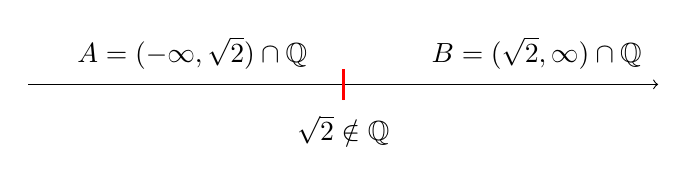
\begin{tikzpicture}
 % Draw a number line
  \draw[->] (-4,0) -- (4,0);
  % Draw a dashed line at 0
  \draw[dashed] (0,-0.2) -- (0,0.2);
  % Label the sets A and B
  \node[anchor=west] at (-3.5,0.4) {$A = (-\infty, \sqrt{2}) \cap \mathbb{Q}$};
  \node[anchor=west] at (1,0.4) {$B = (\sqrt{2}, \infty) \cap \mathbb{Q}$};


  \draw[line width=1pt, red] (0,-0.2) -- (0,0.2);
  \node[anchor=south] at (0,-0.9) {$\sqrt{2} \notin \mathbb{Q}$};
 \end{tikzpicture}
\end{document}